\documentclass[12pt]{article}
\usepackage[T1]{fontenc}
\usepackage{hcmus-report-template}
\usepackage{booktabs,array,tabularx,amssymb}
\input{glyphtounicode}
\pdfgentounicode=1
\setlength{\parindent}{0pt}
\setlength{\parskip}{4pt plus 1pt}
\renewcommand{\baselinestretch}{1.5}
\setlength{\headsep}{12pt}
\setlength{\intextsep}{9pt plus 1pt minus 1pt}
\setlength{\emergencystretch}{1.2em}
\newcolumntype{Y}{>{\raggedright\arraybackslash}X}
\newcommand{\coursename}{CSC14003 -- Nhập môn Trí tuệ Nhân tạo}
\newcommand{\reporttitle}{BÁO CÁO ĐỒ ÁN THỰC HÀNH 2}
\newcommand{\reportname}{Griductive Solver: Suy luận Không Đoán Mò bằng Mã hóa CNF và Bộ giải DPLL}
\newcommand{\leftfooter}{Nhóm thực hiện -- Lớp 24TN (CSC14003)}
\lhead{\small\reporttitle}
\rhead{\small Trường Đại học Khoa học Tự nhiên -- ĐHQG HCM\\\coursename}
\lfoot{\small\leftfooter}
\renewcommand{\refname}{Tài liệu tham khảo}
\floatname{algorithm}{Thuật toán}
\hypersetup{urlcolor=blue,pdftitle={Griductive Solver},pdfauthor={Nhóm thực hiện -- Lớp 24TN},bookmarksnumbered=true}
\algrenewcommand\algorithmicrequire{\textbf{Đầu vào:}}
\algrenewcommand\algorithmicif{\textbf{nếu}}
\algrenewcommand\algorithmicthen{\textbf{thì}}
\algrenewcommand\algorithmicelse{\textbf{ngược lại}}
\algrenewcommand\algorithmicend{\textbf{kết thúc}}
\algrenewcommand\algorithmicfor{\textbf{với}}
\algrenewcommand\algorithmicloop{\textbf{lặp}}
\algrenewcommand\algorithmicwhile{\textbf{trong khi}}
\algrenewcommand\algorithmicdo{\textbf{làm}}
\begin{document}
\pagenumbering{roman}
\hypersetup{pageanchor=false}
\begin{titlepage}
\newcommand{\HRule}{\rule{\linewidth}{0.5mm}}
\centering
\textsc{\LARGE đại học quốc gia tphcm}\\[0.5cm]
\textsc{\Large trường đại học khoa học tự nhiên}\\[0.5cm]
\textsc{\large khoa công nghệ thông tin}\\[0.5cm]
\textsc{bộ môn công nghệ tri thức}\\[0.5cm]
\HRule \\[0.4cm]
{\huge\bfseries\reporttitle}\\[0.5cm]
{\Large\bfseries\reportname}\\[0.4cm]
\HRule \\[0.65cm]
{\large\bfseries Môn học: \coursename}\\[0.7cm]
\begin{minipage}[t]{0.55\textwidth}
\raggedright\emph{Sinh viên thực hiện}\\[3pt]
\begin{tabular}{@{}l@{\quad}r@{}}
Phan Ngọc Thức & 24120228\\
Nguyễn Lê Minh Quân & 24120219\\
Tống Phúc Thiện & 24120141\\
Bùi Phương Nam & 24120502\\
Phan Gia Phúc & 24120503
\end{tabular}
\end{minipage}\hfill
\begin{minipage}[t]{0.40\textwidth}
\raggedleft\emph{Lớp học phần: 24TN}\\[3pt]
Khoa Công nghệ Thông tin
\end{minipage}

\vfill
{\large Thành phố Hồ Chí Minh, ngày 27 tháng 11 năm 2026}\\[0.65cm]

\includegraphics[width=.23\textwidth]{img/hcmus-logo.png}
\vfill
\end{titlepage}

\setcounter{page}{2}
\hypersetup{pageanchor=true}
\setcounter{tocdepth}{2}
{\setstretch{1.05}\tableofcontents}
\clearpage
\listoftables
\clearpage
\listoffigures
\clearpage
\pagenumbering{arabic}
\setcounter{page}{1}
\section{Kế hoạch dự án, phân công và kiến trúc hệ thống}

<<<<<<< HEAD
Một lượt chơi chỉ hợp lệ khi người chơi hoặc tác tử chứng minh được trạng thái của một nhân vật từ những lá bài đã mở. Nhóm triển khai cùng một quy tắc cho chế độ chơi thủ công, chức năng gợi ý và chế độ tự động giải, theo yêu cầu của đồ án CSC14003 \cite{csc14003_spec}. Cách lật thẻ và chọn lời khai tham khảo Griductive và Clues by Sam \cite{griductive_game,cluesbysam}.
=======
Trong Griductive, người chơi chỉ mở được một thẻ nghi phạm khi trạng thái của nhân vật đó là hệ quả logic bắt buộc từ các dữ kiện đã mở. Nhóm xây dựng chương trình áp dụng chung quy tắc không đoán mò này cho thao tác chơi tay, gợi ý và tự động giải theo đề bài CSC14003 \cite{csc14003_spec}, kết hợp tham khảo cách lật thẻ và tô sáng vùng của Griductive và Clues by Sam \cite{griductive_game,cluesbysam}.
>>>>>>> e95a2af30fd2e650472e82590bb55816b145db80

\subsection{Kế hoạch thực hiện và mức độ hoàn thành}

Nhóm thống nhất trước giao diện dữ liệu giữa bàn chơi và bộ suy luận để phát triển song song ba mô-đun lõi (hệ thống vùng, mã hóa CNF và DPLL). Sau khi ghép nối và đối chiếu với bộ đánh giá ngữ nghĩa trực tiếp, nhóm hoàn thiện giao diện Desktop, đo thực nghiệm sáu màn chơi rồi tổng hợp báo cáo và dựng video.

\begin{table}[H]
\centering\small\singlespacing
\caption{Phân công theo mô-đun và tỷ lệ hoàn thành}
\smallskip
\renewcommand{\arraystretch}{1.23}
\begin{tabularx}{\linewidth}{@{}l l >{\raggedright\arraybackslash}X r@{}}
\toprule
\textbf{Thành viên} & \textbf{MSSV} & \textbf{Phần việc phụ trách} & \textbf{Hoàn thành} \\
\midrule
Phan Ngọc Thức & 24120228 & Kiến trúc dự án, giao diện Desktop Cozy Harbor, thực nghiệm, báo cáo và video. & 100\% \\
Nguyễn Lê Minh Quân & 24120219 & Chạy thực nghiệm, đối sánh hai chiến lược chọn biến, phân tích số liệu, báo cáo và video. & 100\% \\
Tống Phúc Thiện & 24120141 & Hệ thống vùng và phép tập hợp, hàm đánh giá ngữ nghĩa, \texttt{GameEngine} và kiểm tra nghiệm duy nhất. & 100\% \\
Bùi Phương Nam & 24120502 & Bộ giải DPLL với hai chiến lược chọn biến và suy luận phản chứng của \texttt{LogicAgent}. & 100\% \\
Phan Gia Phúc & 24120503 & Cổng Tseitin, bộ đếm ngưỡng quy hoạch động và biên dịch toàn bộ mẫu manh mối sang CNF. & 100\% \\
\bottomrule
\end{tabularx}
\end{table}

<<<<<<< HEAD
Tỷ lệ hoàn thành trong bảng được các thành viên thống nhất và ghi nhận tại \texttt{docs/team.json}. Theo công thức tính điểm cá nhân bằng điểm nhóm nhân với tỷ lệ hoàn thành, với mức 100\%, mỗi thành viên nhận trọn điểm nhóm.
=======
Bảng trên khớp với \texttt{docs/team.json}. Điểm cá nhân bằng điểm nhóm nhân với tỷ lệ hoàn thành (ví dụ điểm nhóm 9,0 với mức 90\% nhận 8,1 điểm). Cả năm thành viên hoàn thành trọn phần việc nên cùng đạt 100\%.
>>>>>>> e95a2af30fd2e650472e82590bb55816b145db80

\begin{center}\fbox{\begin{minipage}{.91\linewidth}
\textbf{Video trình diễn trên Google Drive}\\
Liên kết xem:\par{\footnotesize\url{https://drive.google.com/file/d/1Y-84FGh__BUx-dtXgX3oKmJwhWga77Ou/view?usp=sharing}}
\end{minipage}}\end{center}

\clearpage

\subsection{Phân tách dữ liệu ẩn, công khai và luồng xử lý}

\begin{table}[H]
\centering\small\singlespacing
\caption{Trách nhiệm và phạm vi dữ liệu của từng thành phần}
\smallskip
\renewcommand{\arraystretch}{1.23}
\begin{tabularx}{\linewidth}{@{}l >{\raggedright\arraybackslash}X@{}}
\toprule
\textbf{Thành phần} & \textbf{Dữ liệu nắm giữ và nhiệm vụ} \\
\midrule
<<<<<<< HEAD
\texttt{GameEngine} & Giữ \texttt{PrivatePuzzle}, nghiệm đầy đủ, lời khai chưa mở và nhật ký các bước đã chấp nhận; tạo bản sao trạng thái công khai để kiểm tra từng yêu cầu. \\
\texttt{PublicState} & Đối tượng bất biến chứa thông tin bàn, nhân vật, các trạng thái đã biết và lời khai đã mở; các cấu trúc dữ liệu lồng bên trong cũng ở dạng bất biến (\texttt{freeze}). \\
\texttt{LogicAgent} & Chỉ nhận trạng thái công khai và bộ xử lý luật; dựng KB, gọi SAT và chứng minh hoặc từ chối phán quyết. \\
Giao diện Desktop & Cửa sổ PySide6 (Cozy Harbor) điều phối phiên trên worker nền và vẽ lại bàn từ dữ liệu công khai. \\
=======
\texttt{GameEngine} & Giữ đối tượng \texttt{PrivatePuzzle} gồm đáp án ẩn, các lời khai chưa mở và nhật ký nước đi hợp lệ. Trích xuất trạng thái công khai ở mỗi lượt kiểm tra. \\
\texttt{PublicState} & Cấu trúc bất biến chứa kích thước bàn, danh sách nhân vật, các trạng thái đã chứng minh và lời khai đã lật. Các từ điển và danh sách con đều bị khóa sửa đổi. \\
\texttt{LogicAgent} & Chỉ nhận \texttt{PublicState} và bộ đăng ký luật chơi để tạo công thức CNF, gọi DPLL và kết luận chấp nhận hay bác bỏ phán quyết. \\
Giao diện Desktop & Ứng dụng PySide6 (Cozy Harbor) gửi yêu cầu suy luận qua luồng nền và cập nhật hiển thị hoàn toàn dựa trên dữ liệu công khai. \\
>>>>>>> e95a2af30fd2e650472e82590bb55816b145db80
\bottomrule
\end{tabularx}
\end{table}

<<<<<<< HEAD
Khi người chơi gửi một phán quyết, engine chuyển trạng thái công khai hiện tại cho một tác tử kiểm chứng độc lập. Chỉ sau khi có chứng minh, engine mới đối chiếu nghiệm riêng để phát hiện dữ liệu bất nhất, ghi trạng thái, mở lời khai và thêm một bước vào nhật ký; mọi đề nghị bị bác đều không làm lộ nội dung thẻ.

Trong giao diện, \texttt{EngineWorker} chạy hàng đợi tuần tự trong \texttt{QThread} và gửi kết quả về cửa sổ qua signal của Qt \cite{qtforpython6}. Mỗi tác vụ chạy trên bản sao \texttt{GameEngine.fork()}, dùng chung câu đố bất biến nhưng tách riêng trạng thái, lời khai đã mở và danh sách nhật ký. Khi đổi màn hoặc hủy yêu cầu, cờ hủy được kiểm tra cả trong DPLL lẫn trước khi ghi phán quyết để \texttt{SolverCancelled} dừng phép tìm kiếm cũ, đồng thời mã phiên (\texttt{generation}) và mã yêu cầu giúp cửa sổ bỏ qua các kết quả đến muộn.
=======
Khi người chơi chọn phán quyết cho một ô đang úp, \texttt{GameEngine} trích xuất \texttt{PublicState} hiện thời chuyển cho một \texttt{LogicAgent} kiểm chứng độc lập. Chỉ khi phán quyết được chứng minh là bắt buộc, engine mới đối chiếu đáp án gốc để phòng dữ liệu lỗi, mở lời khai của ô đó và ghi thêm một bước vào nhật ký. Mọi nước đi chưa đủ cơ sở hoặc mâu thuẫn đều giữ nguyên bàn và không làm lộ lời khai ẩn.

Để giao diện không bị khựng trên bàn $5\times5$, \texttt{EngineWorker} xử lý tuần tự các yêu cầu trong \texttt{QThread} riêng và báo kết quả qua signal của Qt \cite{qtforpython6}. Mỗi tác vụ chạy trên bản sao \texttt{GameEngine.fork()}, chia sẻ câu đố gốc nhưng tách riêng trạng thái và nhật ký. Khi đổi màn hoặc bấm làm lại giữa chừng, cờ hủy dừng DPLL bằng \texttt{SolverCancelled}, còn cặp mã phiên và mã yêu cầu giúp cửa sổ bỏ qua kết quả cũ đến muộn.
>>>>>>> e95a2af30fd2e650472e82590bb55816b145db80

Giao diện đồ họa, công cụ thực nghiệm dòng lệnh và bộ kiểm thử tự động đều gọi chung lớp kiểm chứng này nên thứ tự mở thẻ và nhật ký suy luận luôn khớp nhau trên cùng tệp câu đố.

\clearpage
\section{Mô hình hóa bài toán và ngôn ngữ manh mối}

\subsection{Biến chính và tri thức công khai}

Trên bàn $N\times N$, với $N\in\{3,4,5\}$, cột A có chỉ số $c=1$ và hàng trên cùng có $r=1$. Biến $C_i$ mang giá trị True (Criminal, tội phạm) hoặc False (Innocent, vô tội), với chỉ số $i=(r-1)N+c$ chạy từ 1 đến $N^2$ (chẳng hạn A3 trên bàn $3\times3$ là biến số 7). Tên và nghề nghiệp chỉ dùng để hiển thị nhận diện nhân vật, còn mọi lời khai đã mở đều luôn đúng kể cả khi chủ thẻ là tội phạm.

Gọi $L_t$ là tập lời khai đã mở và $S_t$ là tập ô đã biết ở bước $t$. Với mỗi ô trong $S_t$, đặt $\ell_i=C_i$ nếu ô là tội phạm và $\ell_i=\neg C_i$ nếu ô vô tội. Cơ sở tri thức (KB) có dạng

\[
KB_t=\bigwedge_{q\in L_t}\operatorname{CNF}(q)\ \land\ \bigwedge_{i\in S_t}(\ell_i).
\]

Tác tử duyệt các ô chưa mở theo thứ tự hàng, chọn ô đầu tiên có phán quyết bắt buộc. Khi engine chấp nhận, trạng thái và lời khai của ô cùng gia nhập KB ở bước kế tiếp. Vòng lặp dừng khi mở hết bàn, hết phán quyết chứng minh được hoặc gặp mâu thuẫn.

\begin{table}[H]
\centering\small\singlespacing
\caption{Sáu kiểu manh mối cơ sở}
\smallskip
\renewcommand{\arraystretch}{1.23}
\begin{tabularx}{\linewidth}{@{}l >{\raggedright\arraybackslash}X@{}}
\toprule
\textbf{Kiểu} & \textbf{Nội dung trên một phép gán} \\
\midrule
\texttt{FACT} & Một người có trạng thái chỉ định, biểu diễn bằng $C_i$ hoặc $\neg C_i$. \\
\texttt{SAME} & Hai người cùng trạng thái, $C_i\leftrightarrow C_j$. \\
\texttt{DIFFERENT} & Hai người khác trạng thái, $C_i\oplus C_j$. \\
\texttt{EXACTLY} & Số tội phạm trong vùng $R$ đúng bằng $k$. \\
\texttt{AT\_LEAST} & Có ít nhất $k$ tội phạm trong $R$. \\
\texttt{AT\_MOST} & Có nhiều nhất $k$ tội phạm trong $R$. \\
\bottomrule
\end{tabularx}
\end{table}

Các manh mối đếm yêu cầu $k$ nguyên và $0\le k\le |R|$. Câu “không có tội phạm” tương ứng với $\operatorname{EXACTLY}(0,R)$. Với vùng rỗng, số tội phạm bằng 0.

\clearpage

\subsection{Vùng, so sánh và điều kiện lồng}

\begin{table}[H]
\centering\small\singlespacing
\caption{Vùng cơ sở và các phép hợp thành}
\smallskip
\renewcommand{\arraystretch}{1.23}
\begin{tabularx}{\linewidth}{@{}l >{\raggedright\arraybackslash}X@{}}
\toprule
\textbf{Kiểu vùng} & \textbf{Tập ô được chọn} \\
\midrule
\texttt{ROW}, \texttt{COLUMN} & Toàn bộ một hàng hoặc một cột hợp lệ. \\
\texttt{NEIGHBORS} & Các ô kề theo tám hướng, bỏ ô mốc. Một ô góc có ba láng giềng, ô biên còn lại có năm và ô ở trong có tám. \\
\texttt{EXPLICIT} & Các ô phân biệt được liệt kê theo định danh. Danh sách có thể rỗng. \\
\texttt{CORNERS} & Bốn ô góc của bàn. \\
\texttt{UNION}, \texttt{INTERSECTION} & Hợp hoặc giao của hai vùng con. Mỗi ô chỉ xuất hiện một lần trong vùng kết quả. \\
\texttt{DIFFERENCE} & Các ô thuộc vùng trái và không thuộc vùng phải. Thứ tự hai toán hạng quyết định kết quả. \\
\bottomrule
\end{tabularx}
\end{table}

\texttt{COMPARISON} so sánh số tội phạm trong hai vùng bằng một trong sáu quan hệ $=,\ne,<,\le,>,\ge$. Nếu hai vùng giao nhau, cùng một biến ô tham gia vào cả hai tổng. \texttt{CONDITIONAL} nhận hai manh mối bất kỳ làm tiền đề và kết luận. Hai vế có thể tiếp tục chứa điều kiện lồng. Mệnh đề kéo theo sai đúng trong trường hợp tiền đề đúng và kết luận sai.

Trong màn \texttt{case-3x3-01}, lời khai công khai B1 đòi hỏi ít nhất ba tội phạm trong tập láng giềng của A2 sau khi trừ hàng 2. Trên bàn này, vùng còn lại là $\{\mathrm{A1},\mathrm{B1},\mathrm{A3},\mathrm{B3}\}$. Cách phân giải vùng xác định chính xác bốn biến đi vào bộ đếm và bốn ô giao diện cần tô sáng.

Bộ đăng ký ánh xạ tên kiểu JSON sang lớp xử lý. \texttt{@register\_region} gắn kiểu vùng với hàm phân giải, còn \texttt{@register\_clue} gắn kiểu manh mối với kiểm tra tham số, biểu thức logic và hàm đánh giá. Gốc có độ sâu 0. Bộ kiểm tra từ chối cây vùng hoặc cây điều kiện khi độ sâu vượt 12. Nhờ giao diện chung, thêm luật mới chỉ cần đăng ký lớp xử lý và kiểm thử ngữ nghĩa của luật đó.

\clearpage
\section{Biểu diễn logic tự động và chuyển đổi sang CNF}

\subsection{Biến đổi các manh mối quan hệ hai ngôi}

Mọi lời khai đang mở đều được biên dịch tự động sang CNF thay vì viết sẵn công thức theo màn. Với \texttt{SAME}, quan hệ tương đương $C_A\leftrightarrow C_B$ được tách thành hai chiều kéo theo rồi áp dụng $p\to q\equiv \neg p\lor q$:

\[
\begin{aligned}
\operatorname{SAME}(A,B)&\equiv C_A\leftrightarrow C_B\\
&\equiv(C_A\to C_B)\land(C_B\to C_A)\\
&\equiv(\neg C_A\lor C_B)\land(C_A\lor\neg C_B).
\end{aligned}
\]

Với \texttt{DIFFERENT}, điều kiện hai người trái trạng thái tương đương có ít nhất một người là tội phạm và không thể cả hai cùng là tội phạm:

\[
\begin{aligned}
\operatorname{DIFFERENT}(A,B)&\equiv C_A\oplus C_B\\
&\equiv (C_A\lor C_B)\land\neg(C_A\land C_B)\\
&\equiv (C_A\lor C_B)\land(\neg C_A\lor\neg C_B).
\end{aligned}
\]

\subsection{Ví dụ mã hóa đếm tổ hợp trực tiếp trên vùng nhỏ}

Xét vùng ba biến $\{A,B,C\}$ với yêu cầu đúng $k=2$ tội phạm. Để có ít nhất 2 tội phạm thì mọi cặp 2 ô đều phải chứa ít nhất một biến đúng; để có nhiều nhất 2 thì cả 3 ô không thể cùng đúng:

\[
\begin{aligned}
\operatorname{EXACTLY}(2,\{A,B,C\})\equiv{}&
(A\lor B)\land(A\lor C)\land(B\lor C)\\
&{}\land(\neg A\lor\neg B\lor\neg C).
\end{aligned}
\]

Tổng quát trên vùng $n$ ô, mã hóa tổ hợp trực tiếp sinh $\binom{n}{n-k+1}=\binom{n}{k-1}$ mệnh đề dương và $\binom{n}{k+1}$ mệnh đề âm, cộng lại là $\binom{n}{k-1}+\binom{n}{k+1}$ mệnh đề (bằng 0 ngoài miền chỉ số). Với $n=25,\ k=12$, riêng một lời khai đã cần $9\,657\,700$ mệnh đề nên không phù hợp cho bàn lớn.

\clearpage
\begingroup\setstretch{1.25}

\subsection{Quy hoạch động đếm ngưỡng unary và cổng Tseitin}

Để giữ kích thước CNF bậc đa thức $O(n^2)$ và tái sử dụng cho phép so sánh vùng, \texttt{Encoder} lập bảng quy hoạch động các ngưỡng unary $T(i,k)$ — mệnh đề “ít nhất $k$ trong $i$ ô đầu của vùng là tội phạm”, với $T(i,0)=\mathrm{True}$ và $T(i,k)=\mathrm{False}$ khi $k>i$. Khi thêm ô thứ $i$ ($C_i$), ngưỡng $k$ đạt được nếu $i-1$ ô trước đã đạt $k$, hoặc đã đạt $k-1$ và $C_i$ đúng:

\[
T(i,k)\leftrightarrow T(i-1,k)\lor\bigl(C_i\land T(i-1,k-1)\bigr).
\]

Mỗi ô $(i,k)$ tạo tối đa một cổng \texttt{AND} và một cổng \texttt{OR} hai đầu vào. Biến phụ được cấp từ $N^2+1$ trong một \texttt{Encoder} chung cho cả $KB_t$; hàm \texttt{gate()} rút gọn hằng, khử literal lặp, triệt tiêu cặp đối dấu và tra bảng băm để dùng lại cổng trùng nhau.

Theo phép biến đổi Tseitin \cite{tseitin1983complexity}, đầu ra phụ được ràng buộc hai chiều để an toàn cả dưới phép phủ định. Với $z\leftrightarrow(a\land b)$ và $w\leftrightarrow(a\lor b)$, ta có:

\[
\begin{aligned}
&(\neg z\lor a)\land(\neg z\lor b)\land(z\lor\neg a\lor\neg b),\\
&(w\lor\neg a)\land(w\lor\neg b)\land(\neg w\lor a\lor b).
\end{aligned}
\]

<<<<<<< HEAD
Đặt $T_R(k)=T(|R|,k)$. Ba ràng buộc “ít nhất”, “nhiều nhất” và “đúng bằng” lần lượt nhận literal hoặc biểu thức $T_R(k)$, $\neg T_R(k+1)$ và $T_R(k)\land\neg T_R(k+1)$. Trong cài đặt thực tế, cả các manh mối hai ngôi như \texttt{SAME} và \texttt{DIFFERENT} cũng được biểu diễn qua \texttt{Encoder.gate} để kết hợp trực tiếp bên trong manh mối điều kiện. Bộ mã hóa buộc đầu ra của mỗi manh mối công khai bằng một mệnh đề đơn; đầu ra hằng sai sinh mệnh đề rỗng, còn đầu ra hằng đúng không cần thêm mệnh đề.
=======
Đặt $T_R(k)=T(|R|,k)$. Ba mẫu \texttt{AT\_LEAST}, \texttt{AT\_MOST} và \texttt{EXACTLY} lần lượt trả về $T_R(k)$, $\neg T_R(k+1)$ và $T_R(k)\land\neg T_R(k+1)$. Đầu ra mỗi lời khai công khai được ép bằng một mệnh đề đơn (nếu hằng sai thì thêm mệnh đề rỗng, hằng đúng thì bỏ qua).
>>>>>>> e95a2af30fd2e650472e82590bb55816b145db80

\subsection{Mã hóa các manh mối mở rộng và kiểm chứng độc lập}

Trong \texttt{COMPARISON}, số tội phạm của $R_1$ lớn hơn hoặc bằng $R_2$ khi mọi ngưỡng $k\ge 1$ đạt ở $R_2$ đều đạt ở $R_1$:

\[
\bigwedge_{k=1}^{|R_2|}\bigl(\neg T_{R_2}(k)\lor T_{R_1}(k)\bigr).
\]

Hoán vị hai vùng cho $\le$, lấy hội hai chiều cho $=$, và phủ định để được $\ne$, $<$ hoặc $>$. Với \texttt{CONDITIONAL}, bộ mã hóa đệ quy lấy hai đầu ra $r_{\mathrm{if}},r_{\mathrm{then}}$ rồi ghép cổng $\neg r_{\mathrm{if}}\lor r_{\mathrm{then}}$. Độc lập với CNF, mỗi lớp đều có hàm \texttt{evaluate()} tính trực tiếp trên phép gán đầy đủ để kiểm thử chéo.

\par\endgroup

\clearpage
\section{Thuật toán DPLL, suy luận phản chứng và kiểm tra nghiệm duy nhất}

\subsection{Thủ tục tìm mô hình DPLL}

Bộ giải trong \texttt{sat.py} được nhóm tự cài đặt theo thuật toán DPLL \cite{davis1962machine}. Trước khi tìm kiếm, hàm \texttt{solve()} khử literal lặp trong từng mệnh đề, bỏ mệnh đề hằng đúng và ghép các giả định (\texttt{assumptions}) thành mệnh đề đơn. Mỗi nhánh đệ quy dùng bản sao phép gán riêng để cô lập khi quay lui.

\begin{algorithm}[H]
\small\singlespacing
\caption{DPLL-Solve với hai chiến lược chọn biến}
\begin{algorithmic}[1]
\Require Công thức CNF $F$, tổng số biến $m$, phép gán $A$ (khởi tạo rỗng), chiến lược $h$
\Loop
\State Kiểm tra cờ hủy và hạn thời gian; nếu $F$ có mệnh đề rỗng thì trả UNSAT.
\State Thu thập tập $U$ các literal trong mệnh đề đơn; nếu $U=\varnothing$ thì thoát vòng lặp.
\For{mỗi $\ell\in U$}
\State Nếu $\ell$ ngược giá trị trong $A$ thì trả UNSAT; nếu biến chưa gán thì ghi vào $A$ và tăng số lan truyền.
\EndFor
\State Rút gọn $F$ theo $A$: bỏ mệnh đề đã thỏa và xóa literal sai khỏi mệnh đề còn lại.
\EndLoop
\If{$F$ rỗng}
\State Điền False cho mọi biến chưa gán trong $1,\ldots,m$; trả SAT kèm mô hình.
\EndIf
\State Đếm tần suất xuất hiện (gộp cả hai dấu) của từng biến còn lại trong $F$.
\State Với \texttt{ordered}, chọn chỉ số nhỏ nhất; với \texttt{frequency}, chọn tần suất lớn nhất (hòa chọn chỉ số nhỏ nhất). Gọi biến được chọn là $v$.
\State Tăng bộ đếm quyết định thêm 1.
\For{$b$ lần lượt nhận True, False}
\State Tạo $A' = A \cup \{v \mapsto b\}$, rút gọn $F$ theo $A'$ và gọi đệ quy DPLL-Solve.
\State Nếu nhánh con trả SAT thì trả mô hình; nếu thất bại thì tăng bộ đếm quay lui.
\EndFor
\State Trả UNSAT.
\end{algorithmic}
\end{algorithm}

Hai mệnh đề đơn đối dấu gây xung đột ngay trong vòng lan truyền. Khi $F$ rỗng, điền \texttt{False} cho các biến tự do vẫn bảo toàn nghiệm. Phép gán phân nhánh được ghi thẳng vào $A'$ nên \texttt{propagations} chỉ đếm đúng các phép gán bị ép buộc, còn thời gian được đo riêng cho từng lời gọi SAT.

\clearpage

\subsection{Kiểm chứng phán quyết bằng phản chứng và lưu mô hình nhân chứng}

Trước hết \texttt{LogicAgent} kiểm tra $KB_t$ khả thỏa để loại trường hợp cơ sở tri thức mâu thuẫn. Khi đó, $KB_t\land\neg C_i$ vô nghiệm chứng minh ô $i$ là tội phạm, còn $KB_t\land C_i$ vô nghiệm chứng minh ô $i$ vô tội. Nếu cả hai đều khả thỏa, mỗi mô hình tìm được đóng vai trò nhân chứng (\textit{witness}) cho một khả năng và ô $i$ vẫn ở trạng thái \texttt{UNKNOWN}.

\begin{algorithm}[H]
\small\singlespacing
\caption{Phân loại các ô chưa mở và kiểm chứng đề nghị}
\begin{algorithmic}[1]
\Require Trạng thái công khai \texttt{PublicState}; chế độ phân loại hoặc kiểm chứng literal đề nghị $p$
\State Dựng $KB_t$ và giải một lần; nếu UNSAT thì trả \texttt{INCONSISTENT}.
\If{chế độ \texttt{verify}}
\State Nếu $KB_t\land\neg p$ là UNSAT thì trả \texttt{ACCEPTED}.
\State Nếu $KB_t\land p$ là UNSAT thì trả \texttt{CONTRADICTED}; ngược lại trả \texttt{NOT\_PROVABLE}.
\EndIf
\State Từ mô hình cơ sở, đánh dấu giá trị (\texttt{True}/\texttt{False}) đã xuất hiện của từng biến chính.
\For{mỗi ô chưa mở theo thứ tự hàng}
\State Nếu $C_i$ đã xuất hiện đủ cả hai giá trị \texttt{True} và \texttt{False}, xuất \texttt{UNKNOWN} và sang ô tiếp theo.
\State Gọi $\ell$ là chiều giá trị chưa có mô hình nhân chứng; giải $KB_t\land\ell$.
\If{kết quả là UNSAT}
\State Xuất \texttt{CRIMINAL} nếu $\ell=\neg C_i$, ngược lại xuất \texttt{INNOCENT}.
\Else
\State Cập nhật giá trị của mọi biến chính từ mô hình mới và xuất \texttt{UNKNOWN}.
\EndIf
\EndFor
\end{algorithmic}
\end{algorithm}

Trong \texttt{LogicAgent.\_verdicts}, mô hình cơ sở ban đầu đã cho sẵn một giá trị thỏa mãn tại mọi biến chính, nên mỗi ô chưa mở chỉ cần tối đa một truy vấn SAT bổ sung (hoặc bằng 0 nếu các mô hình trước đã phủ đủ hai chiều). Bộ nhớ nhân chứng này chỉ tồn tại trong phạm vi một lượt duyệt $KB_t$, còn \texttt{verify()} kiểm tra độc lập từng đề nghị gửi lên nên có thể cần cả hai truy vấn giả định.

Với ví dụ $KB=(C_A\lor C_B)\land(\neg C_A\lor C_B)$, giả định $\neg C_B$ kéo theo cả $C_A$ lẫn $\neg C_A$ nên $B$ bắt buộc là tội phạm; trong khi $A$ nhận được cả \texttt{True} lẫn \texttt{False} khi $C_B=\mathrm{True}$, do đó trạng thái của $A$ là \texttt{UNKNOWN} và thẻ $A$ giữ nguyên úp.

\clearpage

\subsection{Vòng lặp mở thẻ, nhật ký suy luận và kiểm tra nghiệm duy nhất}

Hàm \texttt{next\_verdict()} dừng tại ô bắt buộc đầu tiên: \texttt{hint()} trả về ô gợi ý, còn \texttt{step()} gọi \texttt{submit()} để kiểm chứng lại, lật thẻ, ghi nhật ký (số bước, ô, phán quyết, danh sách ID lời khai đang mở, truy vấn SAT và lời khai mới) rồi dùng trạng thái công khai đã cập nhật cho bước kế tiếp. Khi mọi ô chưa mở đều còn \texttt{UNKNOWN}, vòng tự giải dừng mà không đoán mò.

Nhật ký thực tế của \texttt{case-3x3-01} (\texttt{ordered}) minh họa rõ quy trình này: ở bước 1 với hai lời khai B1 và C1, $KB_1$ gồm 9 biến chính, 39 biến phụ và 123 mệnh đề. Truy vấn cơ sở trả SAT, còn giả định $-7$ trả UNSAT sau 46 phép lan truyền và 0 quyết định, qua đó chứng minh A3 là tội phạm và mở lời khai A3 cho bước 2.

Để kiểm định bộ dữ liệu ngoại tuyến, \texttt{check\_uniqueness()} mã hóa toàn bộ $N^2$ lời khai thành $F$. Nếu $F$ vô nghiệm thì trả \texttt{INCONSISTENT}; nếu có mô hình $M$, hàm thêm mệnh đề chặn chỉ trên tập biến chính $P=\texttt{kb.primary.values()}$:

\[
B_M=\bigvee_{v\in P}\begin{cases}\neg v,&M(v)=\mathrm{True},\\v,&M(v)=\mathrm{False}.\end{cases}
\]

Mọi nghiệm của $F\land B_M$ buộc phải khác $M$ ở ít nhất một nhân vật: kết quả UNSAT xác nhận \texttt{UNIQUE}, còn SAT báo đa nghiệm (\texttt{MULTIPLE}). Chỉ chặn biến chính giúp tránh đếm nhầm khác biệt ở biến phụ Tseitin. Khả năng giải tuần tự từ tập mở đầu vẫn được kiểm tra riêng qua vòng suy luận công khai.

\subsection{Bộ kiểm thử tự động}

Lệnh \texttt{python -B -m unittest discover -s tests -v} chạy đạt toàn bộ 87/87 bài kiểm thử trên 13 mô-đun. Nhóm kiểm thử lõi đối chiếu vét cạn \texttt{evaluate()} với CNF, kiểm tra giả định, quay lui, điều kiện lồng, vùng rỗng và đăng ký luật mới; các mô-đun còn lại kiểm tra tính bất biến của \texttt{PublicState}, từ chối nước đoán mò, hủy worker nền, bộ thực nghiệm và giao diện.

\clearpage
\section{Thực nghiệm và đánh giá hai chiến lược chọn biến}

Hai chiến lược chọn biến (\texttt{ordered} và \texttt{frequency}) được chạy tự động trên cùng sáu câu đố chuẩn theo thứ tự cố định, mỗi cấu hình một lượt trên máy Windows 11, Python 3.14.6, CPU Intel Core i5-12450HX. Cột $N$ ký hiệu kích thước lưới $N\times N$.

\begin{table}[H]
\centering\footnotesize\singlespacing
\caption{Trạng thái kết thúc, quy mô KB cuối phiên và số bước suy luận}
\smallskip
\renewcommand{\arraystretch}{1.13}
\begin{tabular*}{\linewidth}{@{\extracolsep{\fill}}llrllrrrr@{}}
\toprule
\textbf{Màn} & \textbf{Chiến lược} & \textbf{N} & \textbf{Trạng thái} & \textbf{Nghiệm} & \textbf{Biến chính} & \textbf{Biến phụ} & \textbf{Mệnh đề} & \textbf{Bước} \\
\midrule
case-3x3-01 & ordered & 3 & SOLVED & UNIQUE & 9 & 156 & 491 & 7 \\
case-3x3-01 & frequency & 3 & SOLVED & UNIQUE & 9 & 156 & 491 & 7 \\
case-3x3-02 & ordered & 3 & SOLVED & UNIQUE & 9 & 144 & 455 & 7 \\
case-3x3-02 & frequency & 3 & SOLVED & UNIQUE & 9 & 144 & 455 & 7 \\
case-4x4-01 & ordered & 4 & SOLVED & UNIQUE & 16 & 364 & 1138 & 13 \\
case-4x4-01 & frequency & 4 & SOLVED & UNIQUE & 16 & 364 & 1138 & 13 \\
case-4x4-02 & ordered & 4 & SOLVED & UNIQUE & 16 & 273 & 862 & 13 \\
case-4x4-02 & frequency & 4 & SOLVED & UNIQUE & 16 & 273 & 862 & 13 \\
case-5x5-01 & ordered & 5 & SOLVED & UNIQUE & 25 & 668 & 2068 & 22 \\
case-5x5-01 & frequency & 5 & SOLVED & UNIQUE & 25 & 668 & 2068 & 22 \\
case-5x5-02 & ordered & 5 & SOLVED & UNIQUE & 25 & 654 & 2045 & 22 \\
case-5x5-02 & frequency & 5 & SOLVED & UNIQUE & 25 & 654 & 2045 & 22 \\
\bottomrule
\end{tabular*}
\end{table}

\begin{table}[H]
\centering\footnotesize\singlespacing
\caption{Chi phí tìm kiếm DPLL và thời gian chạy của từng cấu hình}
\smallskip
\renewcommand{\arraystretch}{1.13}
\begin{tabular*}{\linewidth}{@{\extracolsep{\fill}}llrrrrr@{}}
\toprule
\textbf{Màn} & \textbf{Chiến lược} & \textbf{Gọi SAT} & \textbf{Quyết định} & \textbf{Lan truyền} & \textbf{Quay lui} & \textbf{Thời gian (s)} \\
\midrule
<<<<<<< HEAD
case-3x3-01 & ordered & 34 & 48 & 2944 & 4 & 0,047 \\
case-3x3-01 & frequency & 33 & 40 & 2942 & 4 & 0,060 \\
case-3x3-02 & ordered & 30 & 34 & 2802 & 15 & 0,071 \\
case-3x3-02 & frequency & 30 & 27 & 2693 & 9 & 0,051 \\
case-4x4-01 & ordered & 84 & 518 & 29666 & 444 & 1,015 \\
case-4x4-01 & frequency & 85 & 287 & 18887 & 8 & 0,504 \\
case-4x4-02 & ordered & 93 & 168 & 12568 & 7 & 1,151 \\
case-4x4-02 & frequency & 91 & 158 & 12567 & 16 & 1,090 \\
case-5x5-01 & ordered & 162 & 193 & 43608 & 18 & 3,483 \\
case-5x5-01 & frequency & 164 & 247 & 44288 & 45 & 3,591 \\
case-5x5-02 & ordered & 182 & 752 & 55976 & 113 & 6,432 \\
case-5x5-02 & frequency & 182 & 647 & 53655 & 37 & 5,540 \\
=======
case-3x3-01 & ordered & 34 & 48 & 2944 & 4 & 0.0469 \\
case-3x3-01 & frequency & 33 & 40 & 2942 & 4 & 0.0598 \\
case-3x3-02 & ordered & 30 & 34 & 2802 & 15 & 0.0708 \\
case-3x3-02 & frequency & 30 & 27 & 2693 & 9 & 0.0511 \\
case-4x4-01 & ordered & 84 & 518 & 29666 & 444 & 1.0145 \\
case-4x4-01 & frequency & 85 & 287 & 18887 & 8 & 0.5043 \\
case-4x4-02 & ordered & 93 & 168 & 12568 & 7 & 1.1509 \\
case-4x4-02 & frequency & 91 & 158 & 12567 & 16 & 1.0898 \\
case-5x5-01 & ordered & 162 & 193 & 43608 & 18 & 3.4830 \\
case-5x5-01 & frequency & 164 & 247 & 44288 & 45 & 3.5915 \\
case-5x5-02 & ordered & 182 & 752 & 55976 & 113 & 6.4323 \\
case-5x5-02 & frequency & 182 & 647 & 53655 & 37 & 5.5400 \\
>>>>>>> e95a2af30fd2e650472e82590bb55816b145db80
\bottomrule
\end{tabular*}
\end{table}

<<<<<<< HEAD
Tổng truy vấn gồm cả tác tử đề xuất và engine kiểm chứng; thời gian bao gồm dựng KB và thực hiện vòng mở thẻ (làm tròn đến ba chữ số thập phân từ kết quả gốc tại \texttt{output/experiments/results.json}). Các phép giải ngoại tuyến để kiểm tra nghiệm duy nhất diễn ra sau khi dừng đồng hồ và được loại khỏi cả bốn bộ đếm.
=======
Số gọi SAT và các bộ đếm gộp cả truy vấn tìm bước của \texttt{LogicAgent} lẫn truy vấn xác minh trong \texttt{GameEngine.submit}. Thời gian làm tròn $10^{-4}$ giây từ \texttt{results.json}; phép kiểm tra \texttt{check\_uniqueness} chạy sau khi dừng đồng hồ nên không tính vào các bộ đếm trên.
>>>>>>> e95a2af30fd2e650472e82590bb55816b145db80

\clearpage

\subsection{So sánh hành vi phân nhánh trên cùng câu đố}

\begin{figure}[H]
\centering
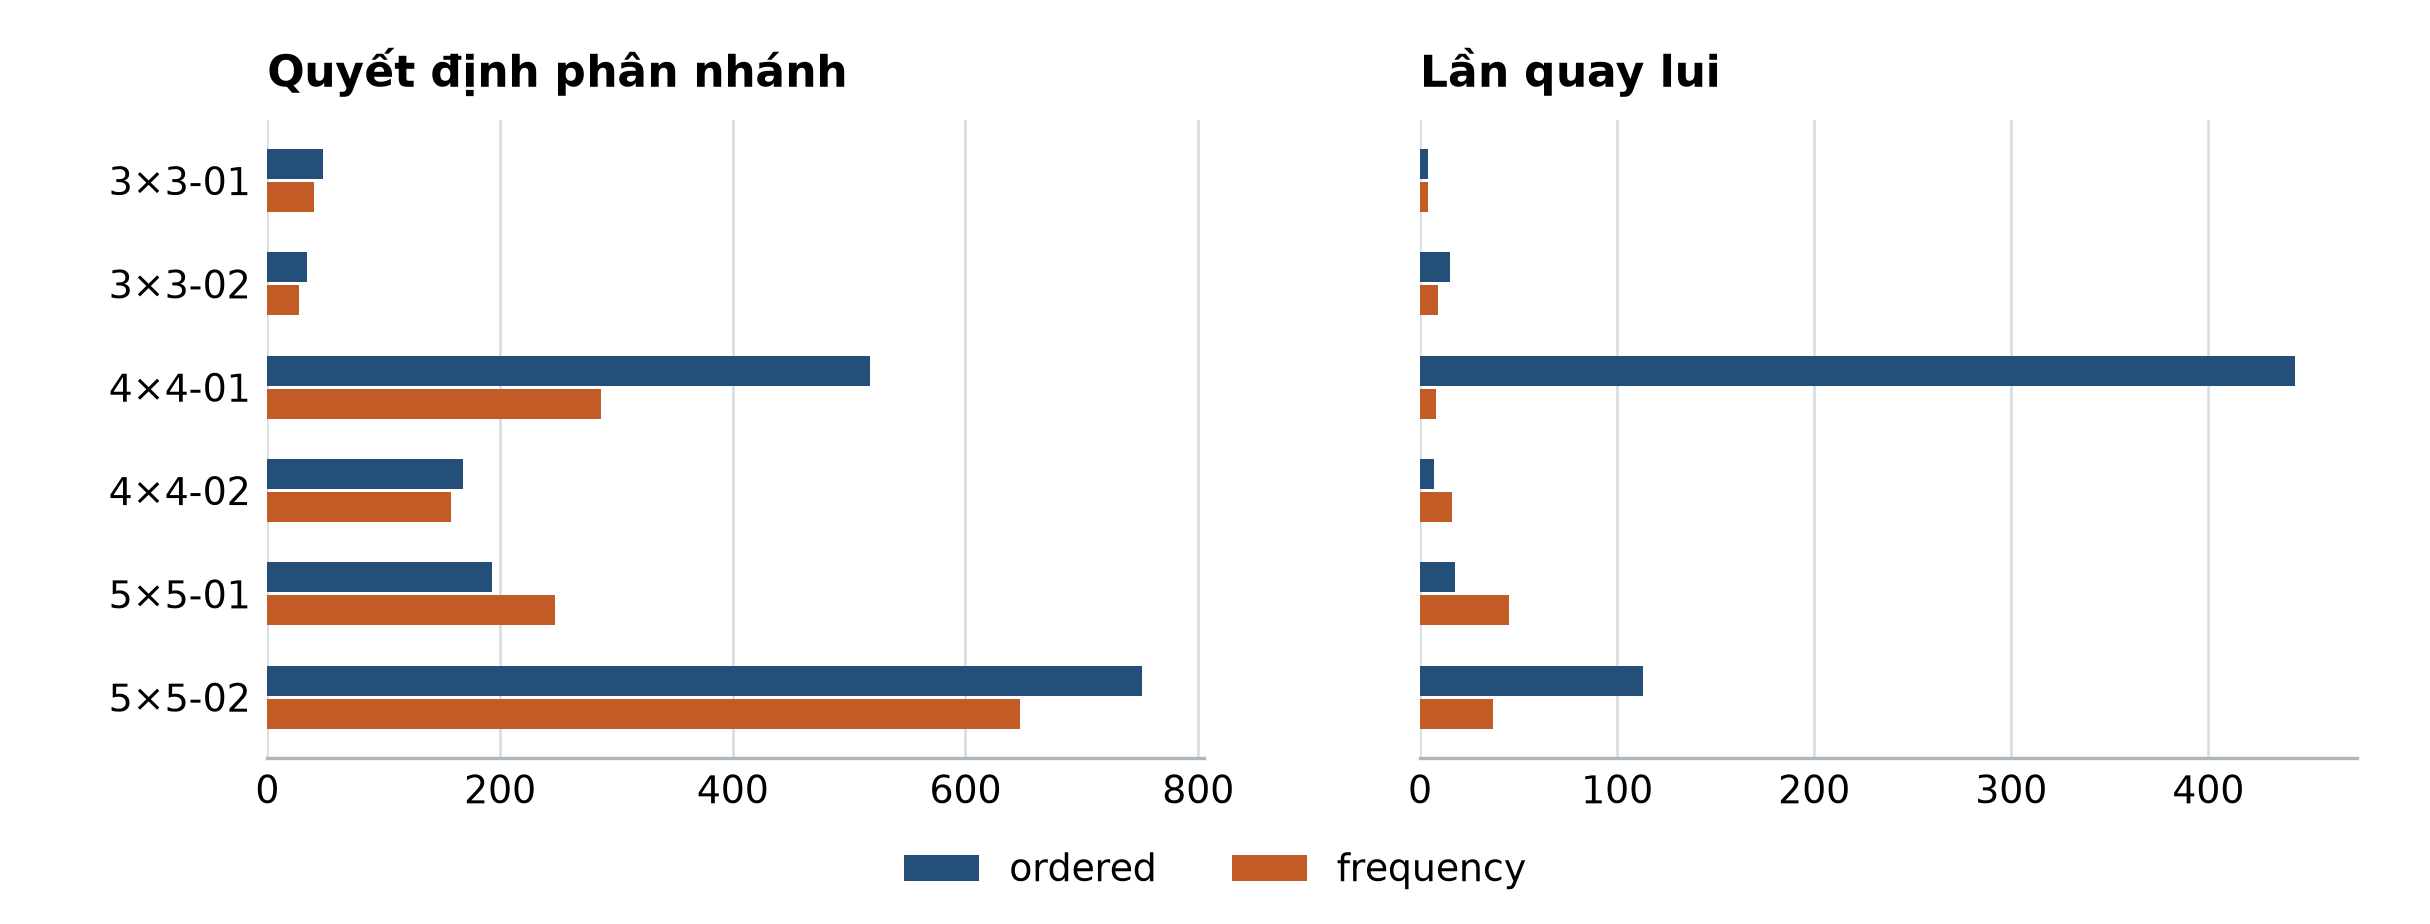
\includegraphics[width=1\linewidth]{img/chart_decisions_backtracks.png}
\caption{Số quyết định phân nhánh và số lần quay lui của hai chiến lược (hai trục ngang dùng thang riêng).}
\end{figure}

<<<<<<< HEAD
Trên màn $4\times4$-01, chuyển sang \texttt{frequency} giúp giảm từ 518 xuống 287 quyết định và từ 444 xuống 8 lần quay lui, dù số lần gọi SAT tăng nhẹ từ 84 lên 85. Trong lần giải KB ban đầu, \texttt{ordered} chọn biến số 1 (xuất hiện 4 lần trong công thức đã rút gọn), trong khi \texttt{frequency} chọn biến số 11 — một biến ô trên bàn $4\times4$ xuất hiện tới 24 lần. Gán biến liên quan đến nhiều mệnh đề có thể buộc thêm các ngưỡng đếm và làm lộ xung đột sớm.
=======
Khác biệt rõ nhất nằm ở \texttt{case-4x4-01}: chuyển sang \texttt{frequency} giảm từ 518 xuống 287 quyết định và từ 444 xuống 8 lần quay lui, dù số lần gọi SAT tăng từ 84 lên 85. Tại KB đầu tiên, \texttt{ordered} rẽ nhánh vào biến số 1 (xuất hiện 4 lần trong công thức rút gọn), còn \texttt{frequency} chọn biến số 11 (biến ô giao nhiều vùng đếm, xuất hiện 24 lần). Gán sớm biến có độ liên kết cao giúp kích hoạt lan truyền qua các ngưỡng đếm và bộc lộ xung đột nhanh hơn.
>>>>>>> e95a2af30fd2e650472e82590bb55816b145db80

Các biến phụ Tseitin cũng tham gia tính tần suất cùng biến chính. Một biến ngưỡng dùng chung ở nhiều cổng so sánh thường xuất hiện dày và tác động đồng thời lên nhiều ràng buộc. Trên màn \texttt{case-5x5-02}, với cùng 182 lần gọi SAT, \texttt{frequency} giảm từ 752 xuống 647 quyết định, hạ quay lui từ 113 xuống 37 lần và rút ngắn thời gian từ 6,4323 xuống 5,5400 giây.

Ngược lại, ở \texttt{case-5x5-01}, \texttt{ordered} chỉ cần 193 quyết định và 18 lần quay lui trong khi \texttt{frequency} tăng lên 247 và 45. Ngay ở KB mở đầu, \texttt{ordered} chọn biến số 4 và tìm được mô hình sau hai quyết định, còn \texttt{frequency} chọn biến số 18 nhưng nhánh thử \texttt{True} đầu tiên rơi vào ngõ cụt. Vì cả hai luôn thử \texttt{True} trước, ưu tiên tần suất cao vẫn có thể dẫn bộ giải vào nhánh sai trước khi quay lui.

\clearpage
\begingroup\setstretch{1.25}

\subsection{Thời gian chạy, quy mô CNF và hạn chế của hệ thống}

\begin{figure}[H]
\centering
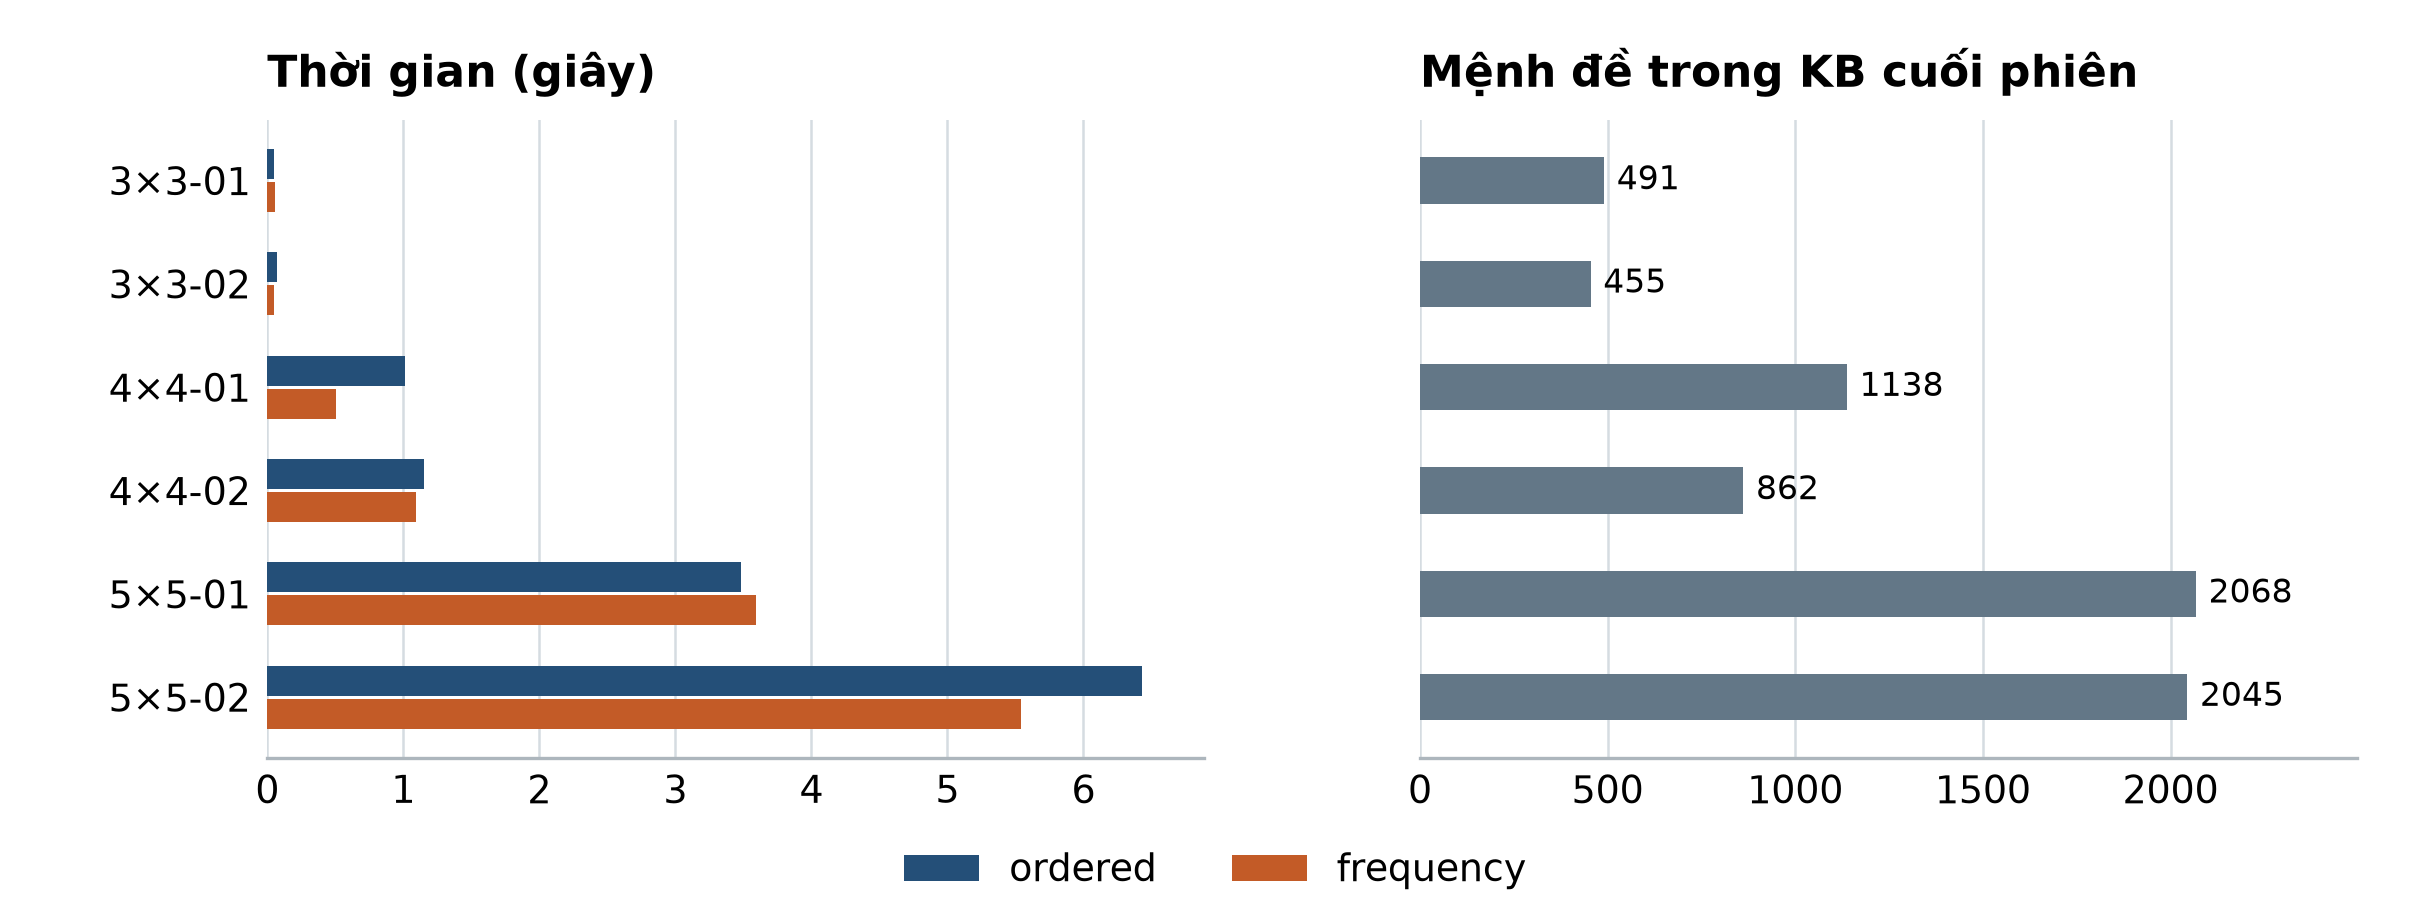
\includegraphics[width=1\linewidth]{img/chart_runtime_clauses.png}
\caption{Thời gian giải toàn màn và tổng số mệnh đề trong KB cuối phiên.}
\end{figure}

Cỡ bàn không quyết định toàn bộ chi phí giải. Hai màn $5\times5$ cùng mở 22 thẻ và có số mệnh đề cuối gần nhau (2\,068 và 2\,045), nhưng \texttt{case-5x5-02} phân nhánh nhiều hơn nên mất 5,54--6,43 giây so với 3,48--3,59 giây của \texttt{case-5x5-01}. Ở \texttt{case-4x4-01}, việc giảm mạnh quay lui giúp \texttt{frequency} rút nửa thời gian (1,0145 xuống 0,5043 giây), còn trên bàn $3\times3$ thời gian dưới 0,08 giây nên chịu ảnh hưởng đáng kể bởi chi phí đếm tần suất và tải hệ thống.

Khi hai chiến lược trả về mô hình cơ sở khác nhau, tập giá trị \texttt{True}/\texttt{False} ghi nhận sẵn cho các biến chính cũng thay đổi, làm số lần gọi SAT đôi khi lệch 1--2 truy vấn dù mở cùng số thẻ. Tại \texttt{case-4x4-02}, \texttt{frequency} giảm quyết định (158 so với 168) nhưng quay lui nhiều hơn (16 so với 7), cho thấy cần đánh giá kết hợp nhiều chỉ số.

Cả 12 lượt đều đạt \texttt{SOLVED} và kiểm tra ngoại tuyến đạt \texttt{UNIQUE}. Nếu gặp màn thiếu dữ kiện hoặc mâu thuẫn, vòng lặp ghi nhận nguyên trạng thái \texttt{UNKNOWN}, \texttt{INCONSISTENT} hoặc \texttt{TIMEOUT} vào bảng kết quả. Hạn mặc định mỗi màn là 30 giây, kiểm tra giữa các bước kèm hạn riêng trên từng truy vấn SAT.

Về hạn chế, DPLL thuần Python hiện quét lại danh sách mệnh đề ở mỗi bước lan truyền và rút gọn, chưa cài đặt kỹ thuật hai literal canh (\emph{two-watched literals}) hay học mệnh đề xung đột như CDCL. Ngoài ra, bộ thực nghiệm mới đo một lượt mỗi cấu hình trên sáu màn nên phù hợp để phân tích hành vi tìm kiếm cụ thể hơn là ước lượng phân bố thống kê trên lưới lớn hơn.

\par\endgroup

\clearpage
\begingroup\setstretch{1.22}
\section{Giao diện người dùng Desktop Cozy Harbor và Web Dash}

\subsection{Chọn màn và chơi thủ công}

Cozy Harbor hiển thị tọa độ, tên, nghề nghiệp, trạng thái đã chứng minh và lời khai trên thẻ đang mở. Từ menu hồ sơ, người chơi chọn một trong sáu màn hoặc mở tệp JSON. Chọn một thẻ úp để gửi phán quyết tội phạm hoặc vô tội. Khi chứng minh thành công, thẻ lật để lộ lời khai tiếp theo.

\begin{figure}[H]
\centering
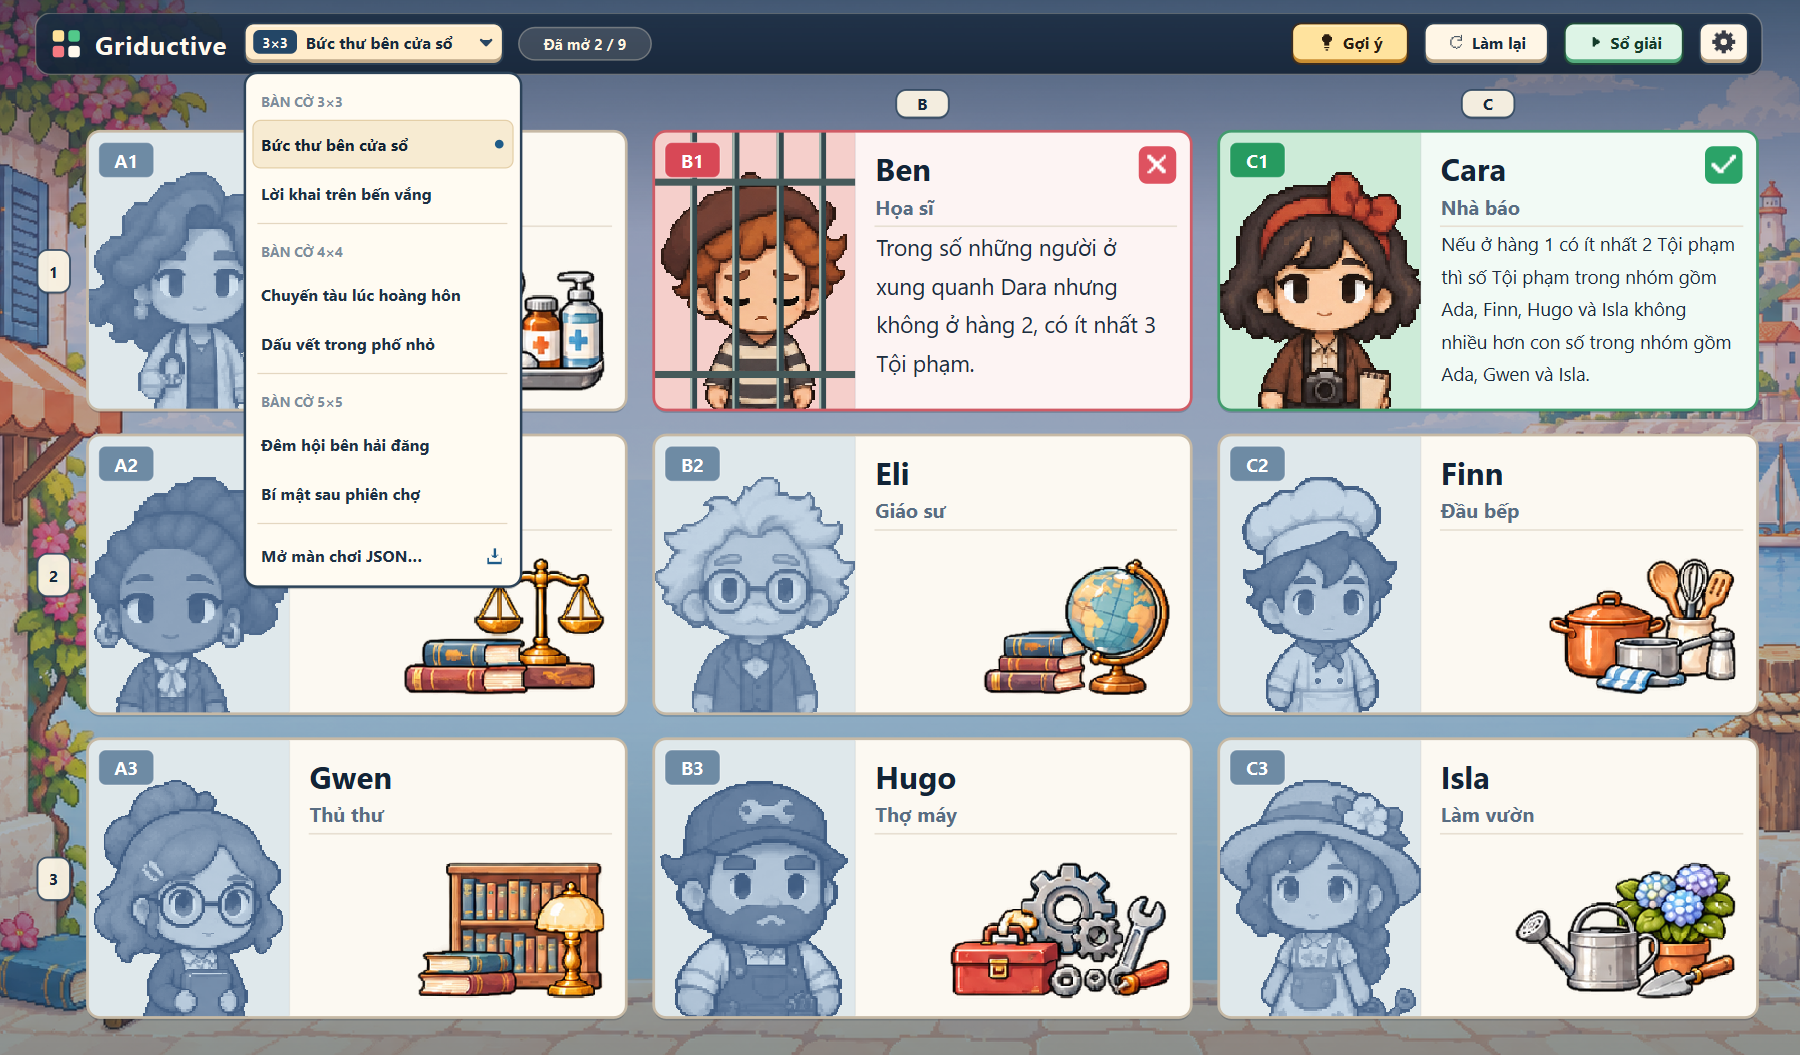
\includegraphics[width=0.78\linewidth]{img/ui_3x3_casemenu.png}
\caption{Menu hồ sơ trên bàn $3\times3$. Các màn được nhóm theo kích thước bàn.}
\end{figure}

Gợi ý xác định nhân vật có thể chứng minh tiếp theo từ cùng ảnh chụp công khai. Nút “Xem nhân vật” dẫn người chơi đến thẻ cần xét. Thao tác xem gợi ý giữ nguyên số thẻ đã mở.

\begin{figure}[H]
\centering
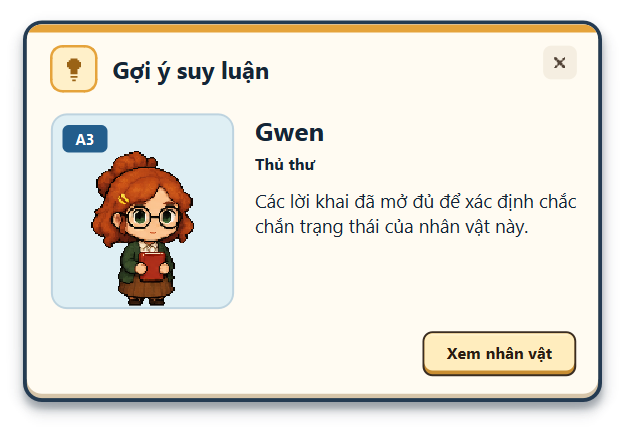
\includegraphics[width=0.34\linewidth]{img/ui_hint_modal.png}
\caption{Hộp gợi ý chỉ đến Gwen, thủ thư ở A3, khi các lời khai đã đủ để xác định trạng thái của cô.}
\end{figure}

\clearpage

\subsection{Đọc lời khai và theo dõi quá trình giải}

\begin{figure}[H]
\centering
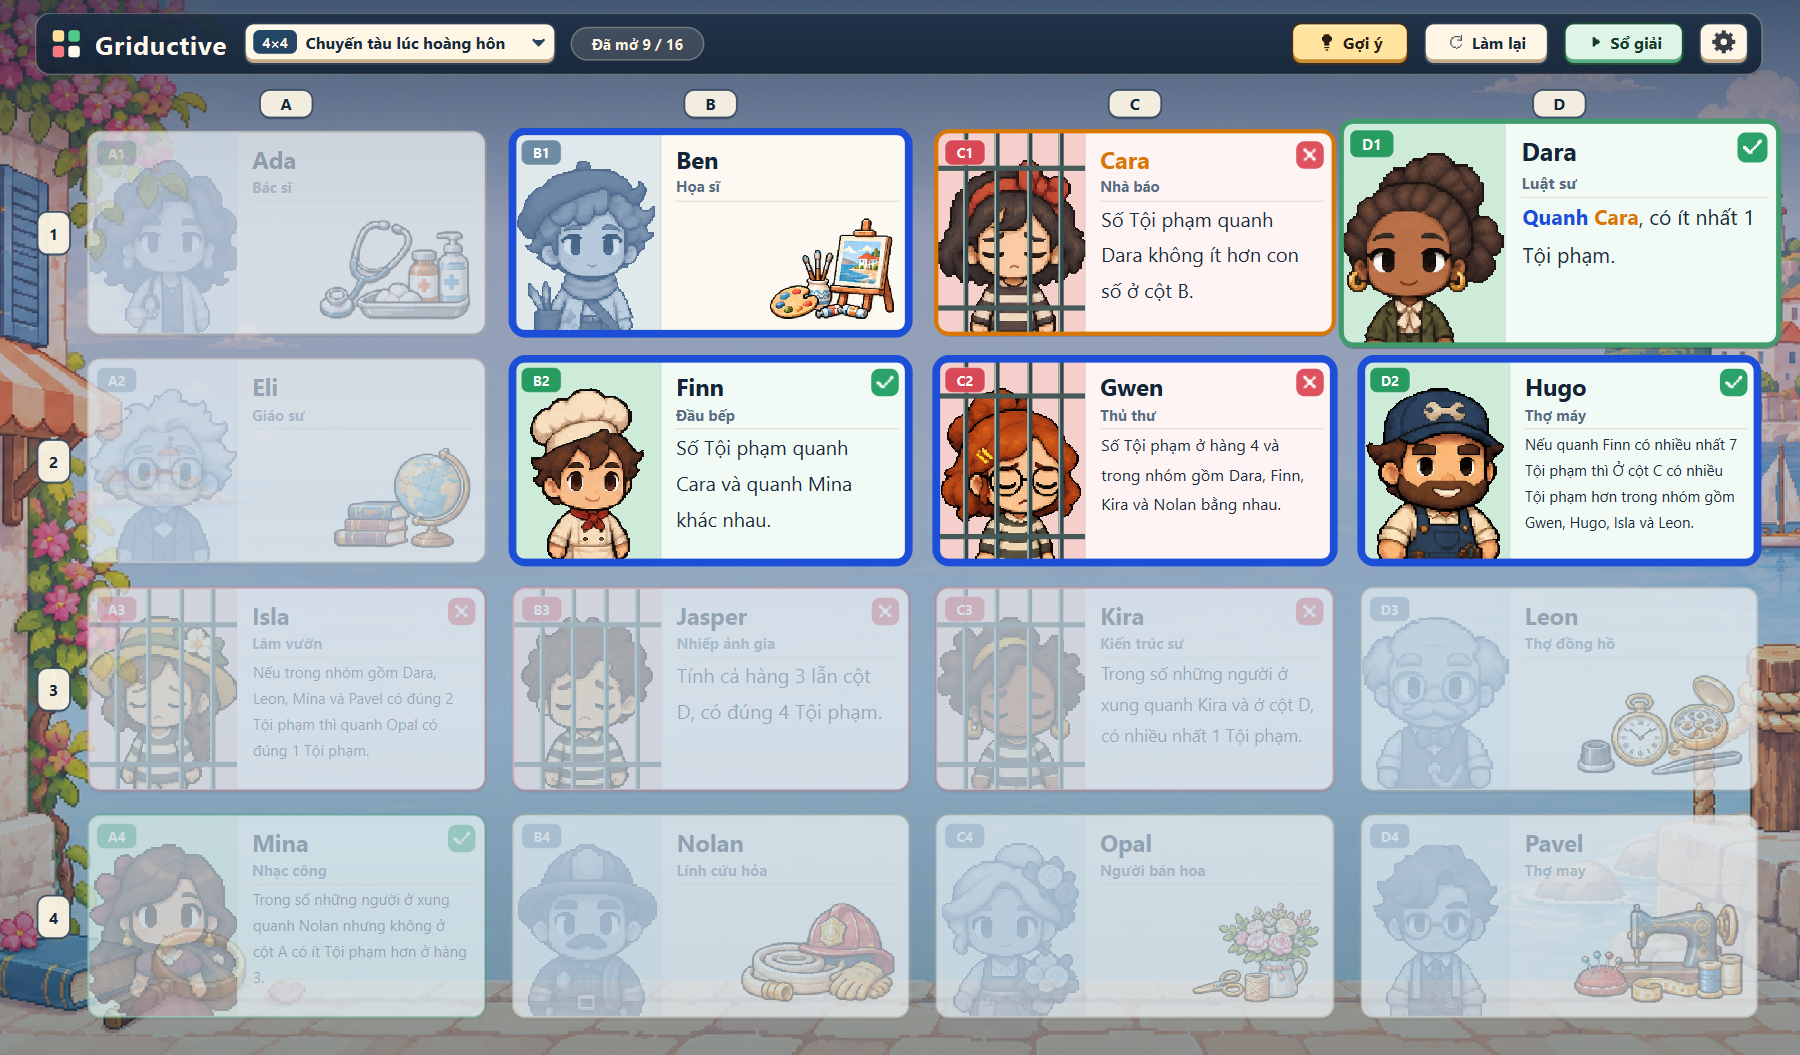
\includegraphics[width=0.75\linewidth]{img/ui_4x4_highlights.png}
\caption{Bàn $4\times4$ khi chọn lời khai. Viền màu xác định các ô thuộc vùng tham chiếu, còn các ô ngoài vùng được làm mờ.}
\end{figure}

Với lời khai nhiều vùng, màu của từng cụm từ khớp với đường viền trên bàn. Chọn hoặc ghim một vùng giúp đọc đúng toán hạng của phép so sánh. “Tự giải” lần lượt thực hiện các bước đã chứng minh. “Làm lại” khởi tạo lại màn từ những thẻ mở ban đầu.

\begin{figure}[H]
\centering
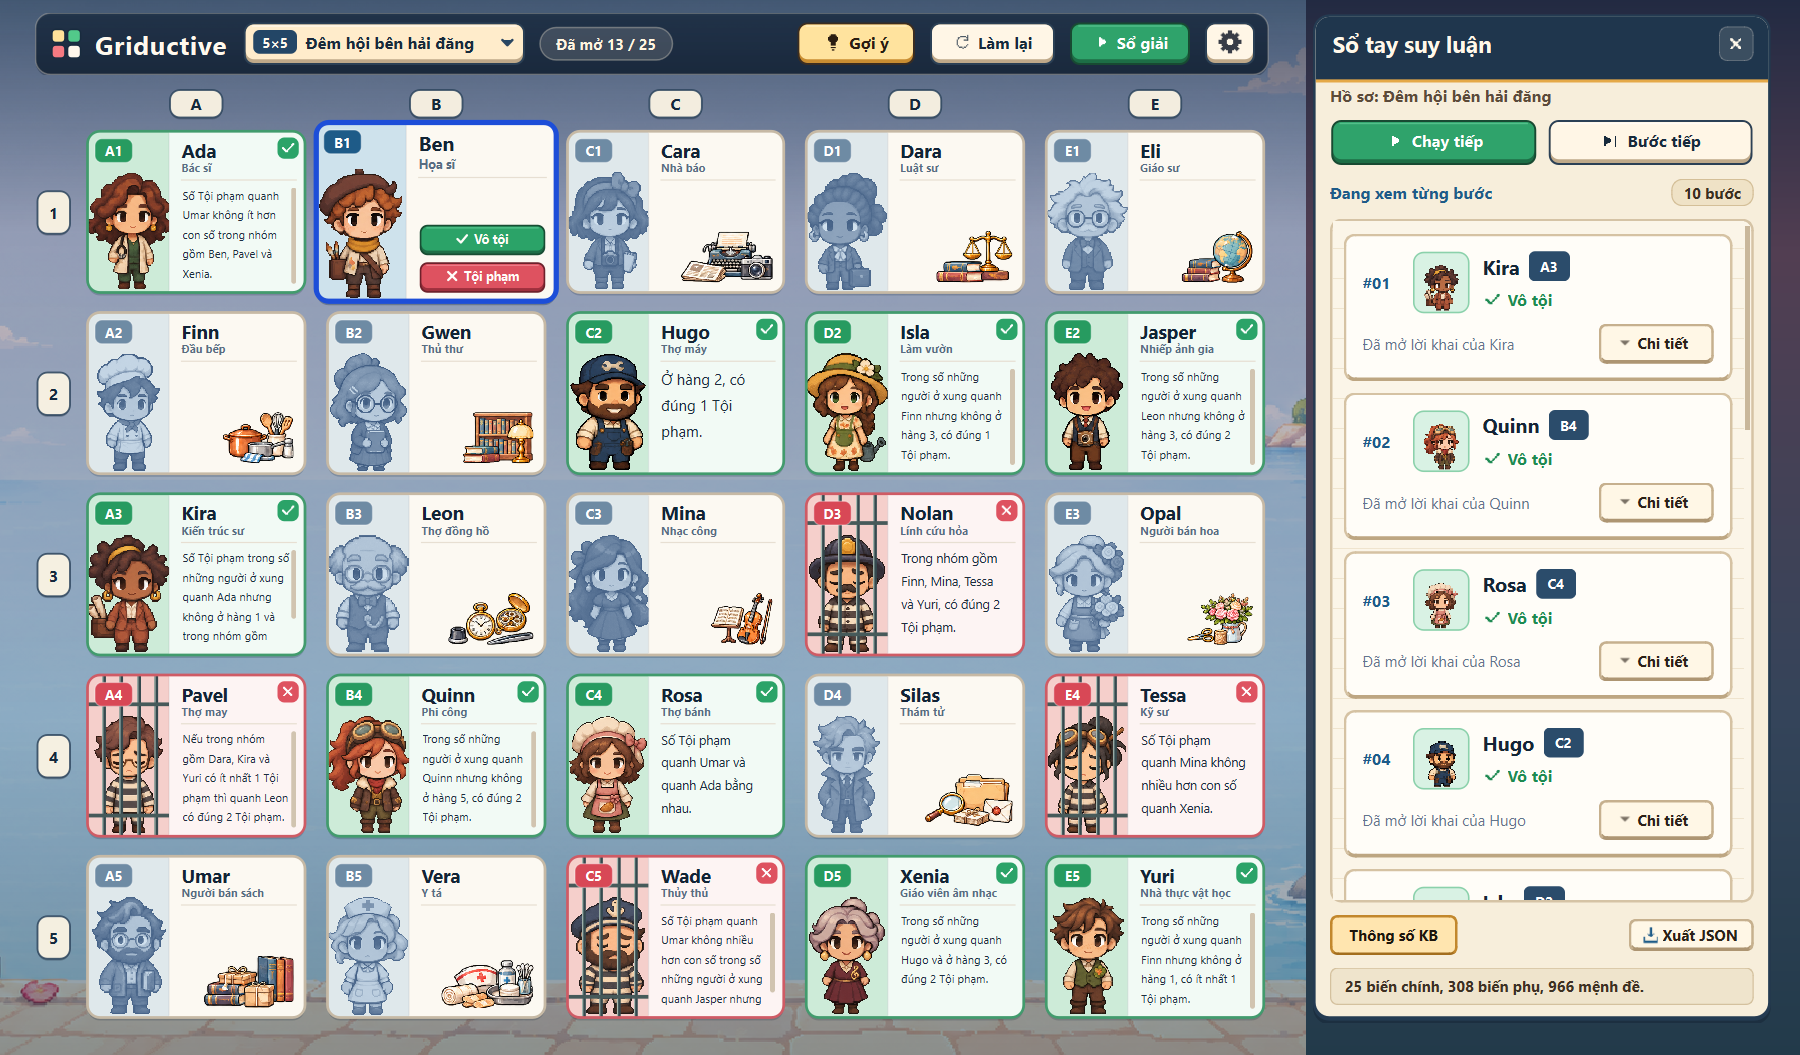
\includegraphics[width=0.75\linewidth]{img/ui_5x5_solver.png}
\caption{Bàn $5\times5$ bên cạnh sổ tay suy luận. Mỗi mục ghi ô vừa được xác định và có nút xem chi tiết.}
\end{figure}

\clearpage

\subsection{Phiên chơi Web Dash}

Giao diện Web dùng callback của Plotly Dash \cite{dashdocs} để nhận thao tác, dựng lại bàn và trả phần hiển thị công khai. Với màn có sẵn, \texttt{dcc.Store} ở chế độ \texttt{session} lưu mã màn, lịch sử nước đi và lựa chọn hiển thị. Đáp án và manh mối chưa mở nằm ở máy chủ. Nếu người chơi tự nạp tệp JSON, dữ liệu phiên còn giữ bản tệp do chính họ cung cấp để tái dựng màn.

Mỗi callback tạo một GameEngine cho phiên, kiểm tra kiểu dữ liệu và giới hạn số nước trong lịch sử theo số ô. Máy chủ phát lại từng đề nghị qua \texttt{submit}. Một nước thiếu chứng minh hoặc bị sửa sẽ khiến lịch sử bị từ chối. Chỉ sau khi tái dựng thành công, callback mới xử lý thao tác mới. Các phiên có thể đọc cùng bộ câu đố bất biến nhưng không chia sẻ tiến độ chơi.

Ví dụ, tự thêm A3 vào lịch sử phía trình duyệt chỉ có hiệu lực nếu máy chủ chứng minh được phán quyết tại đúng thời điểm đó. Đoán đúng đáp án ẩn vẫn chưa đủ để mở lá bài. Bộ kiểm thử Web gửi yêu cầu callback thật, kiểm tra từ chối lịch sử giả và xác nhận dữ liệu trả về cho màn tích hợp sẵn không chứa nghiệm ẩn.

Tệp tùy chỉnh được kiểm tra mã hóa, giới hạn 128 000 byte sau giải mã và được đọc qua một tệp tạm trước khi đưa vào bộ nạp câu đố chung. Cả Desktop và Web đều dùng chung phép chứng minh và điều kiện chấp nhận. Desktop giữ phiên trên worker, còn Web trả chi phí phát lại lịch sử để có thể xử lý yêu cầu kế tiếp trong tiến trình mới.

\par\endgroup

\clearpage
\phantomsection
\addcontentsline{toc}{section}{Tài liệu tham khảo}
\renewcommand{\refname}{Tài liệu tham khảo}
\bibliographystyle{unsrt}
\bibliography{ref/ref}

\clearpage
\appendix
\section{Phụ lục về AI tạo sinh và cách kiểm chứng}

\subsection{Lập trình, tích hợp và soạn báo cáo}

Trong quá trình thực hiện, nhóm tự thiết kế kiến trúc ranh giới công khai/ẩn, đặc tả luật và trực tiếp cài đặt các thuật toán lõi (phân giải vùng, đánh giá ngữ nghĩa, mã hóa CNF và bộ giải DPLL). Nhóm sử dụng Codex và Antigravity như công cụ hỗ trợ gợi ý khung kiểm thử, đối chiếu biên điều kiện và rà soát tính nhất quán cho giao diện cũng như báo cáo. Khi đặt yêu cầu cho công cụ, nhóm luôn nêu rõ ranh giới dữ liệu công khai, đầu ra mong đợi và các trường hợp phải từ chối.

Chẳng hạn, khi rà soát phần suy luận, nhóm đặt yêu cầu: “Chỉ truyền \texttt{PublicState} cho tác tử; với mỗi phán quyết, thử giả định phủ định và làm rõ điều kiện trả về \texttt{UNKNOWN} hoặc \texttt{INCONSISTENT}.” Tương tự, với nhóm luật mở rộng, yêu cầu nêu đủ cả sáu toán tử so sánh và cho phép \texttt{CONDITIONAL} nhận hai cây manh mối bất kỳ. Mọi phần mã và gợi ý thu được đều do nhóm kiểm chứng lại bằng phản ví dụ, đối chiếu phép gán hoàn chỉnh, bộ kiểm thử tự động và nhật ký thực nghiệm chạy trực tiếp trên máy.

\subsection{Đồ họa, sửa ảnh có mặt nạ và nghiệm thu}

Nhật ký \texttt{docs/AI-PROMPTS.md} lưu các prompt tạo atlas, ảnh tham chiếu, lỗi cần chỉnh sửa và thứ tự khung hình. Ở bản phác thảo biểu cảm ban đầu (9 khung cho Ada), nhóm yêu cầu khóa căn chỉnh khung hình với đoạn trích nguyên văn: “keep face center, eye line, head scale, hair silhouette and shoulders in exactly same position across all nine frames”, nhằm tránh tình trạng nhân vật bị nhảy vị trí khi chuyển biểu cảm.

Khi chuyển sang phong cách pixel chính thức với 7 khung hình cho mỗi nhân vật, nhóm chỉ định rõ số hàng/cột, nền RGBA trong suốt, phần trang phục thay đổi, biên mỗi ô và vùng cần để trống cho ImageGen. Với hiệu ứng chớp mắt, Stable Diffusion 1.5 Inpainting chỉ tái tạo vùng mặt nạ quanh mắt, giữ nguyên pixel ngoài mặt nạ và kênh alpha gốc \cite{inpainting}. Khi cập nhật lại 7 khung của nhân vật Finn, nhóm đối chiếu 24 hàng nhân vật còn lại theo từng byte, đồng thời kiểm tra mép alpha và chiều cao tư thế. Toàn bộ ảnh giao diện ở mục 6 là ảnh chụp trực tiếp từ chương trình đang chạy.

\subsection{Thuyết minh và nguồn đối chiếu}

ElevenLabs TTS chuyển kịch bản tiếng Việt thành từng đoạn thoại để khớp với thao tác trên bàn. Quy trình đo thời lượng từng tệp âm thanh, ghép đoạn vào trục hình 24 khung/giây và dùng các khoảng ngắt giọng để căn phụ đề. Các cảnh chọn màn, gợi ý, phán quyết bị từ chối và tự giải được kiểm tra theo trạng thái cửa sổ và thông báo của engine. Âm thanh và hình minh họa phục vụ trình bày, còn phán quyết trong phần mềm luôn xuất phát từ DPLL.

Tài liệu \texttt{docs/REFERENCES.md} ghi phạm vi đã khảo sát. Nhóm tham khảo hướng dẫn thiết kế giao diện trò chơi \cite{gamedev}, đọc phần mô hình và điều phối của clues-by-sam-solver \cite{safina}, đồng thời khảo sát README và cấu trúc hai dự án Griductive \cite{trantai,wadew}. Khi đối chiếu một ý tưởng từ nguồn ngoài, nhóm dùng luật của đề và kết quả thử trên chính mã Python của nhóm để quyết định cách áp dụng.

\end{document}
